{\fontsize{11}{14}\selectfont 

La taratura della bilancia è stata effettuata  prendendo delle masse di cui è noto il valore nominale con più cifre significative della risoluzione della bilancia, per cui il loro errore è stato considerato trascurabile. 
\par
L'intervallo scelto per la taratura della bilancia è entro i 4 grammi, cioè la massima differenza di peso misurata al variare della corrente.
\\
Sono quindi state messe le pesate nella \autoref{fig:GraficoTaratura}.
\par
\begin{figure}[H]
  \centering
  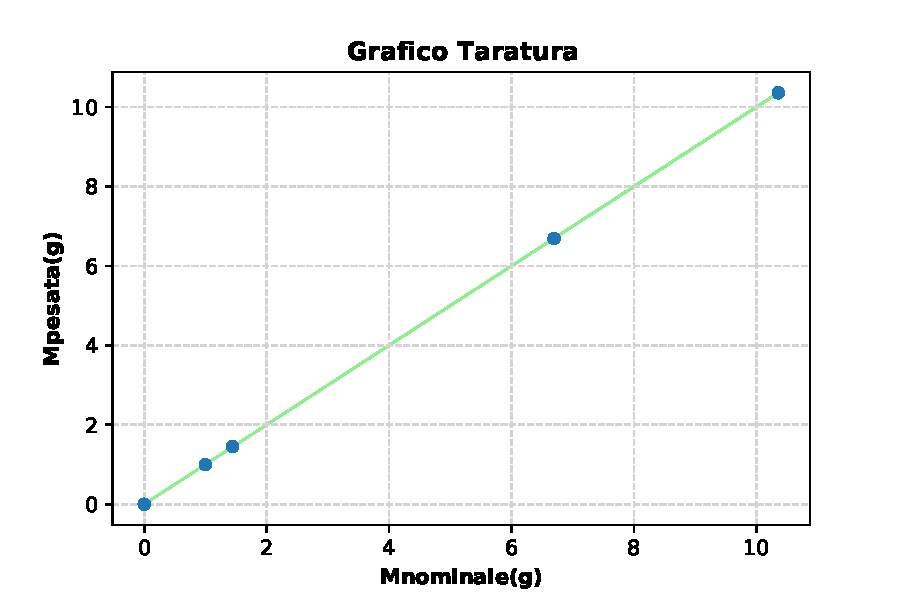
\includegraphics[width=13.5cm]{Figures/Grafico_Taratura.pdf}
  \caption{Grafico della massa pesata sulla massa nominale (entrambe in grammi). L'errore sulla massa nominale è stato considerato trascurabile, mentre l'errore sulla massa pesata è 0.01g. L'andamento è lineare e con pendenza $1$ come ci si aspetta da una bilancia tarata.}   
  \label{fig:GraficoTaratura}
\end{figure}
\par
Da questo grafico è stato possibile ricavare la pendenza attraverso un fit con la seguente formula
\begin{equation*}
    M_{pesata} = \text{pendenza}\cdot M_{nominale}
\end{equation*}
la quale è risultata essere $pendenza = 1.0000 \pm 0.0003$, compatibile con il valore 1. 
\\
In conclusione, la bilancia era tarata opportunamente.
\par}